\documentclass{40k}


\newcommand{\tertiaries}
{%
\missionsubheading{Tertiary Objectives.}  Both players apply all of
the following tertiary objectives.  \underline{No more than~5 total
  victory} \underline{points may be earned by a player across all of
  the tertiary objectives.}

\begin{itemize}
\item \textit{Victory Through Attrition.}  Score~1 victory point for
  each unsaved hull point or wound taken from any opposing superheavy
  vehicle or gargantuan creature by any means, including explosions
  and other indirect effects.  These points are earned at the end of
  any phase in which such damage occurs, and thus include any repaired
  or regenerated later.

\item \textit{Slay the Warlord.}  If the opposing army has a Lord of
  War character or a Warlord of any type and either has been removed
  as a casualty or is falling back at the end of the game, score~2
  victory points.

\item \textit{Linebreaker.}  Score~2 victory points if a model from
  any friendly scoring unit is completely within 12'' of your
  opponent's table edge.

\item \textit{First Blood.}  As defined on page~133 of the main
  \emph{Warhammer 40,000} rulebook.
\end{itemize}
}


%%----------------------------------------------------------------------
%%----------------------------------------------------------------------
\begin{document}

\pagetitle{Mission Pack}

\begin{columns}

\missionheading{Army Construction}

Armies must be selected to at most~\underline{1850 points}.  Players
will use a single army list for all missions.  All up to date
sources\footnote{Partial list maintained by Redcap's Corner and PAGE:
  \url{http://bit.ly/1uWkFHz}} are permitted.  No requirements or
constraints are placed on detachments or force organizations.  Forge
World units and armies eligible for standard \emph{Warhammer 40,000}
are permitted.

Models need not be painted, but objective painting scores will be
applied to reward finished armies.

Models must be WYSIWYG, but identifiable and thoughtful conversions
are welcome.  Contact the tournament organizer(s) beforehand about any
uncertain models.  ``Counts-as'' proxies and undistinguishable or
confusing stand-ins are not permitted.

\missionheading{Supporting Materials}

You must have an official, legal, complete physical or digital copy on
hand for all army, unit, and other sources you are using.  You should
bring printed copies of relevant pages of any electronic sources.
Don't forget errata and FAQs for your sources.\footnote{Available from
  The Black Library:
  \url{http://www.blacklibrary.com/faqs-and-errata.html}}

You must bring any dice, templates, and markers you need to facilitate
playing your army, as well as five typed copies of your army roster
with points listed.


\missionheading{Startup Sequence}
Each mission will use the following setup process:

\begin{itemize}\shortlist
\item Clarify terrain and exchange lists

\item Determine warlord traits, then psychic powers, and then other
  pre-game effects and choices

\item D6 roll off to select deployment zones

\item Place primary objective markers

\item D6 roll off to choose first or second deployment

\item Deploy main armies in that order

\item Deploy any Infiltrators (pg. 167)

\item Secretly choose and record secondary objectives from the options
  listed for the mission

\item Make any Scout redeployments (pg. 171)

\item Reveal secondary objectives

\item First to deploy chooses to play first or second

\item Seize the Initiative roll, if desired

%\item \emph{Fight!}
\end{itemize}

\columnbreak

\missionheading{Mission Rules}%

The following special rules will be applied to each mission, in
addition to any given by the mission definition or otherwise
specified, e.g., for a particular table.

\missionsubheading{Easy Recon.}  Players add~+1 to their roll to
choose first or second deployment for each superheavy vehicle or
gargantuan creature in the opposing army.

\missionsubheading{Reserves.} As defined on page~135 of the main
\emph{Warhammer 40,000} rulebook.

\missionsubheading{Seize the Initiative.} As defined on page~132 of
the main \emph{Warhammer 40,000} rulebook.

\missionsubheading{Variable Game Length.} As defined on page~133 of
the main \emph{Warhammer 40,000} rulebook.

\missionsubheading{All In.}  Units/models in reserve at game end count
as completely destroyed/removed as a casualty.

\missionheading{Scoring}%

Match results are determined by scoring primary, secondary, and
tertiary objectives as given for each mission.  Any unit or faction
specific rules granting victory points \emph{to a player's opponent}
also apply.  The winner is the player with more victory points.

Tournament standings are determined by win/draw/loss records and then
the sum total victory points earned across all three missions.  No
more than~20 victory points may be earned per mission toward these
standings, though any additional victory points do count toward
determining match results.

% Ties are broken in favor of the player with the most army points on
% the table at game end, including embarked units and claimed
% fortifications.

\vfill
\begin{story}{62pt}{The Joy of Flight}
  Kraxxus smiled as he punched the release for the Thunderhawk's rear
  hatch and felt the thin air suddenly gusting throughout the
  transport.  In quick intervals his talon of Raptors launched
  themselves into the sunlight, swirling downward.  Smiling even
  broader, Kraxxus revved his jump pack and ran down the length of the
  bay, throwing himself after his flock in a high speed dive...
\end{story}

\end{columns}

%%----------------------------------------------------------------------
%%----------------------------------------------------------------------
\clearpage
\missiontitle{Table Setup Guide}

The following illustrations are just guides to aid understanding;
consult the rules for details.

\missionheading{Mission 1: Drop Zone}

\bigskip\centerline{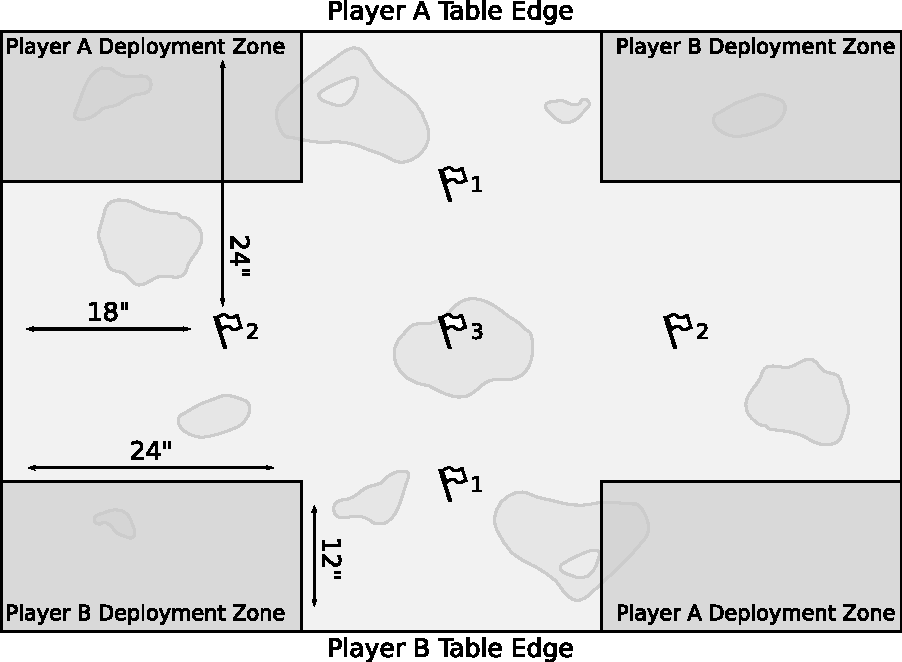
\includegraphics[scale=0.6]{maps/mission1}}

\missionheading{Mission 2: Forced March}

\bigskip\centerline{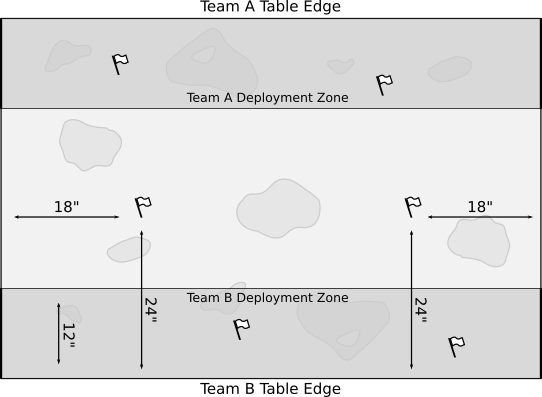
\includegraphics[scale=0.6]{maps/mission2}}

\missionheading{Mission 3: Killing Fields}

\bigskip\centerline{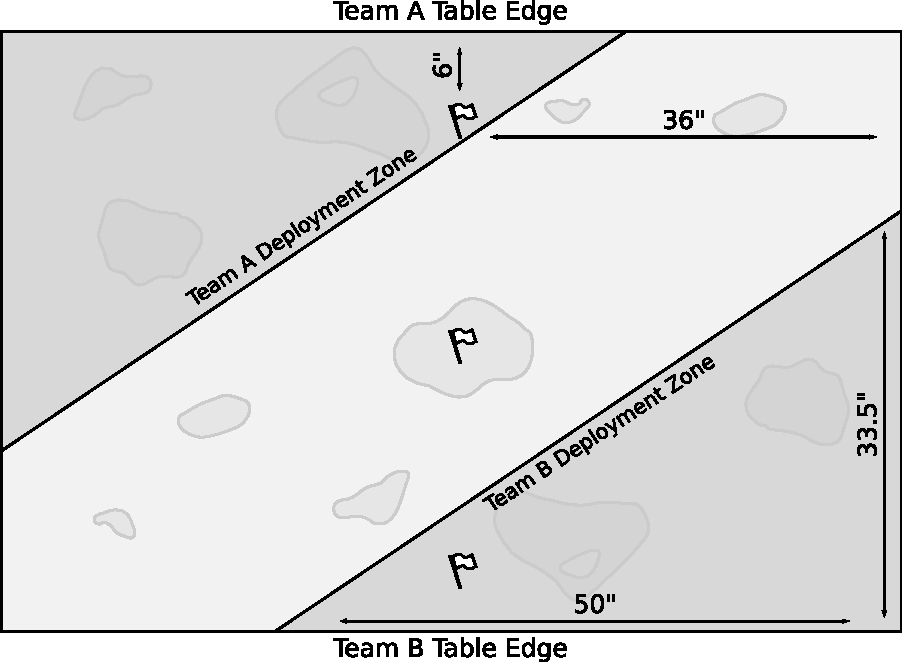
\includegraphics[scale=0.6]{maps/mission3}}

%%----------------------------------------------------------------------
%%----------------------------------------------------------------------
\clearpage
\missiontitle{Mission 1: Drop Zone}

\centerline{\emph{Rapid strike forces land and fight to carve out a
    beachhead for their armies.}}

\missionheading{Table Setup}

Deployment zones are the rectangles in each table corner~12'' in from
the long edge and~24'' in from the short edges.  The player that wins
the zone roll off picks either pair of \emph{diagonally opposite}
corners as their deployment zone and a long table edge as their player
edge.  The other player takes the other pair of diagonally opposite
corners and opposite long edge.

\bigskip%
After determining deployment zones, place five primary objective
markers: One at the center of the table worth~3 victory points; two
more 18'' from the short table edges and 24'' from the long table
edges worth~2 points each; and two~36'' from the short table edges and
12'' from the long table edges worth~1 point each.

\missionheading{Mission Specific Rules}

The following mission specific rules apply, in addition to those
applied to all missions in this pack.

\missionsubheading{Strike Force.}  All Fast Attack units have the
Obective Secured rule, as defined on page~122 of the rulebook.

%\missionsubheading{Nightfighting.}  All units have Stealth on Turn 1.



\missionheading{Scoring}

This mission is scored by objectives achieved, as follows.

\missionsubheading{Primary Objectives.}  Each primary objective marker
is worth their respective value given above.


\missionsubheading{Secondary Objectives.}

After deployment, both players simultaneously choose and then reveal a
single secondary objective for themselves from the list below.  Any
necessary selections are chosen and then revealed with the objective
unless noted otherwise.  \underline{No more than~6 victory points may
  be earned via any secondary.}

\begin{itemize}
\item \textit{Seize Ground.}  Choose two terrain pieces not in your
  deployment zone.  Do not declare these now, but do secretly record
  your selection unambiguously!  Reveal these at game end and score~3
  victory points for each piece that you control, treating them as
  objective markers.  Note that this means a single unit cannot claim
  both a primary objective marker and a terrain piece simultaneously.

\item \textit{Seek and Destroy.}  Choose and declare a Battlefield
  Role other than Troop.  Score~2 victory points for each enemy unit
  of this role completely destroyed or falling back at the end of the
  game.

\item \textit{Assassinate.}  Score~1 victory point for each opposing
  character model removed as a casualty or falling back at the end of
  the game.  Note that this is not limited to just independent
  characters.
\end{itemize}


\tertiaries


%%----------------------------------------------------------------------
%%----------------------------------------------------------------------
\clearpage
\missiontitle{Mission 2: Forced March}

\centerline{\emph{The armies begin the long maneuvers from their drop
    sites to the targets of their campaign.}}

\missionheading{Table Setup}

Deployment zones are \textbf{Hammer and Anvil}, as defined on page~131
of the main rulebook (24'' short edges).

\bigskip%
In each of the four table corners place a primary objective marker
12'' from both of the table edges of that corner.  Place a fifth
primary objective marker at the center of the table.

\missionheading{Mission Specific Rules}

The following mission specific rules apply, in addition to those
applied to all missions in this pack.

\missionsubheading{The Longest Day.}  After Turn~4 roll a D6; on a~4+
all units have Stealth for the remainder of the game.  Do this again
after Turn~5 if it did not take effect.  This rule automatically takes
effect after Turn~6.


\missionheading{Scoring}

This mission is scored by objectives achieved, as follows.

\missionsubheading{Primary Objectives.} At the conclusion of the game,
players score~1 victory point for each objective they control in their
own deployment zone and~2 points for the marker at table center.
Players earn~3 additional victory points if they control one marker in
the enemy deployment zone, and~5 points if they control both.

\missionsubheading{Secondary Objectives.}

After deployment, both players simultaneously choose and then reveal a
single secondary objective for themselves from the list below.  Any
necessary selections are chosen and then revealed with the objective
unless noted otherwise.  \underline{No more than~6 victory points may
  be earned via any secondary.}

\begin{itemize}
\item \textit{Control the Field.}  Each table quarter in which you
  have a scoring unit and your opponent does not, or you have an
  Objective Secured Unit and your opponent does not, is worth 2
  victory points.

\item \textit{Seek and Destroy.}  Choose and declare a Battlefield
  Role other than Troop.  Score~2 victory points for each enemy unit
  of this role completely destroyed or falling back at the end of the
  game.

\item \textit{Meatgrinder.}  Score~1 victory point for each opposing
  Troop unit destroyed or falling back at game end.

\end{itemize}

\tertiaries

%%----------------------------------------------------------------------
%%----------------------------------------------------------------------
\clearpage
\missiontitle{Mission 3: Killing Fields}

\centerline{\emph{Blow for blow, both sides work simply to eviscerate
    each other's armies.}}

\missionheading{Table Setup}

Deployment zones are \textbf{Vanguard Strike}, as defined on page~131
of the main \emph{Warhammer 40,000} rulebook.  Vanguard Strike may be
approximated by deploying within a 33.5'' x 50'' table corner
triangle.  The player that wins the zone roll off may pick any of the
four corners, and the other player takes that diagonally opposite.

\bigskip%
After determining deployment zones, place one secondary objective
marker at the center of the table and one at each of the two table
quadrant centers outside the deployment zones, i.e., 18'' from the
short table edge and 12'' from the long table edge in the corners
opposite the deployment zones.  There are thus three secondary
objective markers along the diagonal dividing the space between the
two deployment zones.


\missionheading{Mission Specific Rules}

There are no mission specific rules for this mission.


\missionheading{Scoring}

This mission is scored by objectives achieved, as follows.

\missionsubheading{Primary Objectives.}

At game end, victory points are earned by each player as follows:

\begin{squishitemize}
\item At least~1 of your opponent's units has been destroyed: +1

\item The total number of points or units lost by your opponent is
  more than those you lost: +1

\item At least 25\%, 50\%, and 75\% of your opponent's army by points
  or units is destroyed: +2 each quartile

%\item At least 25\% of your opponent's army by points value or number
%  of units has been destroyed: +2
%
%\item At least 50\% of your opponent's army by points value or number
%  of units has been destroyed: +2
%
%\item At least 75\% of your opponent's army by points value or number
%  of units has been destroyed: +2

\item All of your opponent's units have been destroyed: +1

\end{squishitemize}

\missionsubheading{Secondary Objectives.}

After deployment, both players simultaneously choose and then reveal a
single secondary objective for themselves from the list below.  Any
necessary selections are chosen and then revealed with the objective
unless noted otherwise.  \underline{No more than~6 victory points may
  be earned via any secondary.}

\begin{itemize}
\item \textit{Control the Field.}  Each table quarter in which you
  have a scoring unit and your opponent does not, or you have an
  Objective Secured Unit and your opponent does not, is worth 2
  victory points.

\item \textit{Hold the Line.}  Each secondary objective held is
  worth~2 victory points.

% \item \textit{Seize Ground.}  Choose two terrain pieces not in your
%   deployment zone.  Do not declare these now, but do secretly record
%   your selection unambiguously!  Reveal these at game end and score~3
%   victory points for each piece that you control, treating them as
%   objective markers.  Note that this means a single unit cannot claim
%   both a primary objective marker and a terrain piece simultaneously.

\end{itemize}


\tertiaries


\end{document}
